% --------------------------------------------------------------
% This is all preamble stuff that you don't have to worry about.
% Head down to where it says "Start here"
% --------------------------------------------------------------
 
\documentclass[12pt]{article}
 
\usepackage[margin=1.5cm,top=1cm]{geometry} 
\usepackage[utf8]{inputenc}
\usepackage[T1]{fontenc}
\usepackage[dvips]{graphicx}
\usepackage{xcolor}
\usepackage{times}
\usepackage{amsmath,amsthm,amssymb}
\usepackage{dsfont}
\usepackage{slashed}
\usepackage{mathtools}
\usepackage[shortlabels]{enumitem}
\usepackage{tikz}
\usetikzlibrary{calc}
\tikzset{>=latex} 
\usetikzlibrary{decorations.pathmorphing}
\usetikzlibrary{decorations.markings}
\usetikzlibrary{arrows.meta}
\usetikzlibrary{shapes.symbols}



\newenvironment{problem}[2][Problem]{\begin{trivlist}
\item[\hskip \labelsep {\bfseries #1}\hskip \labelsep {\bfseries #2.}]}{\end{trivlist}}

\begin{document}
 
% --------------------------------------------------------------
%                         Start here
% --------------------------------------------------------------
 
\title{Homework 6 Classical Mechanics\\Deadline December 6, 2023.}
\date{}
 
\maketitle


\begin{problem}{1}
Show that in the scattering produced by a repulsive potential energy $U = \alpha E r ^{-2}$
the differential cross section is given by
\begin{equation}
\frac{d\sigma}{d\Omega}=\alpha\pi^2\frac{\pi-\theta}{(2\pi-\theta)^2\theta^2\sin\theta}.
\end{equation}
\end{problem}


\begin{problem}{2}
Consider three equally spaced beads on a ring of radius $a$ as shown in the figure, with $m_1=\mu$ and $m_2 = m_3 =  m$ . Assume the masses are subject to 2-body linear
restoring forces proportional to the change of the angle of separation with spring constants $k_1 = k_3 = k$, $k_2 = \kappa$. The potential
energy is given by
\begin{equation}
U=\frac{k a^2}{2}(\eta_2-\eta_1)^2+\frac{k a^2}{2}(\eta_3-\eta_1)^2+\frac{\kappa a^2}{2}(\eta_2-\eta_3)^2,
\end{equation}
where
\begin{equation}
\eta_1=\theta_1,\quad \eta_2=\theta_2-2\pi/3,\quad\eta_3=\theta_3-4\pi/3.
\end{equation}
Find the frequencies of oscillation, sketch the normal modes, and
construct the modal matrix.


\begin{center}
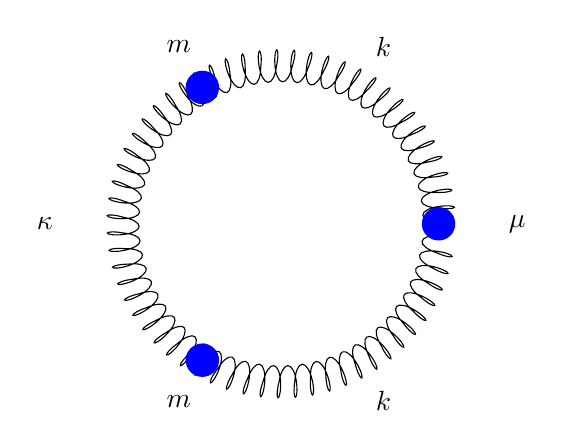
\begin{tikzpicture}
\draw[decoration={aspect=0.3, segment length=2mm, amplitude=2mm,coil},decorate] (2,0) arc (0:360:2);
\node[circle,fill=blue,inner sep=1.5mm] (a) at (2,0) {};
\node at (3,0) {$\mu$};
\node[circle,fill=blue,inner sep=1.5mm] (a) at (-1., 1.73205) {};
\node at (-1.3, 2.25167) {$m$};
\node[circle,fill=blue,inner sep=1.5mm] (a) at (-1., -1.73205) {};
\node at (-1.3, -2.25167) {$m$};
\node at (1.3, 2.25167) {$k$};
\node at (1.3, -2.25167) {$k$};
\node at (-3,0) {$\kappa$};
\end{tikzpicture}
\end{center}

\end{problem}

\begin{problem}{3}
\begin{enumerate}[(a)]
\item Find the inertia tensor of a uniform cube of side $a$ pivoted at one corner and with the edges adjacent to that corner aligned with the axes of an orthonormal coordinate system.
\item Find the principal axis system and the moments of inertia about the pivot.
\end{enumerate}

\end{problem}
\begin{problem}{4}
A uniform hoop of mass $M$ and radius $R$ hangs in a vertical plane supported by a nail at one point inside the circumference. Calculate the natural frequency of small oscillations. 
\begin{center}
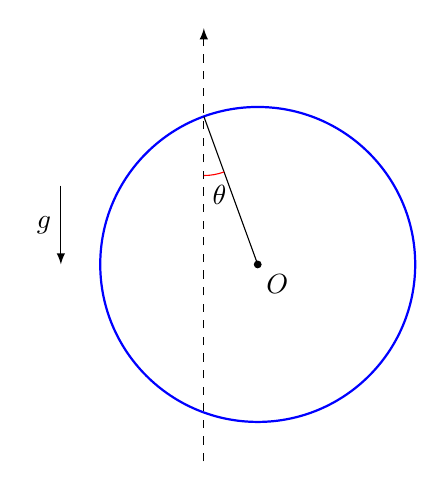
\begin{tikzpicture}[important line/.style={thick,blue},scale=1]
\draw [important line,fill=white,opacity=1] (0,0) circle (2);
\draw[->,dashed] (-0.684,-2.5) -- (-0.684,3); %axis
\draw[-] (-0.684,1.8794) -- (0,0); %axis
\draw (-0.484,0.8794) node{$ \theta $}; % theta
\draw (0.25,-0.25) node{$ O $}; 
\node at (0,0)[circle,fill,inner sep=1pt] {};
\draw[->] (-2.5,1) -- node[left] {$g$}(-2.5,0) ;
\draw[red] (-0.684,1.1294) arc (-90:-70:0.75);
\end{tikzpicture}
\end{center}

\end{problem}


 
\end{document}